%
% $RCSfile: web_user_interface.tex,v $
%
% Copyright (c) 2002-2007. Christian Heller. All rights reserved.
%
% Permission is granted to copy, distribute and/or modify this document
% under the terms of the GNU Free Documentation License, Version 1.1 or
% any later version published by the Free Software Foundation; with no
% Invariant Sections, with no Front-Cover Texts and with no Back-Cover
% Texts. A copy of the license is included in the section entitled
% "GNU Free Documentation License".
%
% http://www.cybop.net
% - Cybernetics Oriented Programming -
%
% Version: $Revision: 1.2 $ $Date: 2007-08-01 13:59:01 $ $Author: christian $
% Authors: Christian Heller <christian.heller@tuxtax.de>
%

\subsection{Web User Interface}
\label{web_user_interface_heading}
\index{Web User Interface}

A \emph{Web User Interface} (WUI) is what is commonly also known as
\emph{Hypertext Markup Language} (HTML) file. HTML files get interpreted by a
\emph{Web Browser} which renders the graphical and textual information to
display these as HTML page. Figure \ref{web_user_interface_figure} shows an
example WUI.

\begin{figure}[ht]
    \begin{center}
        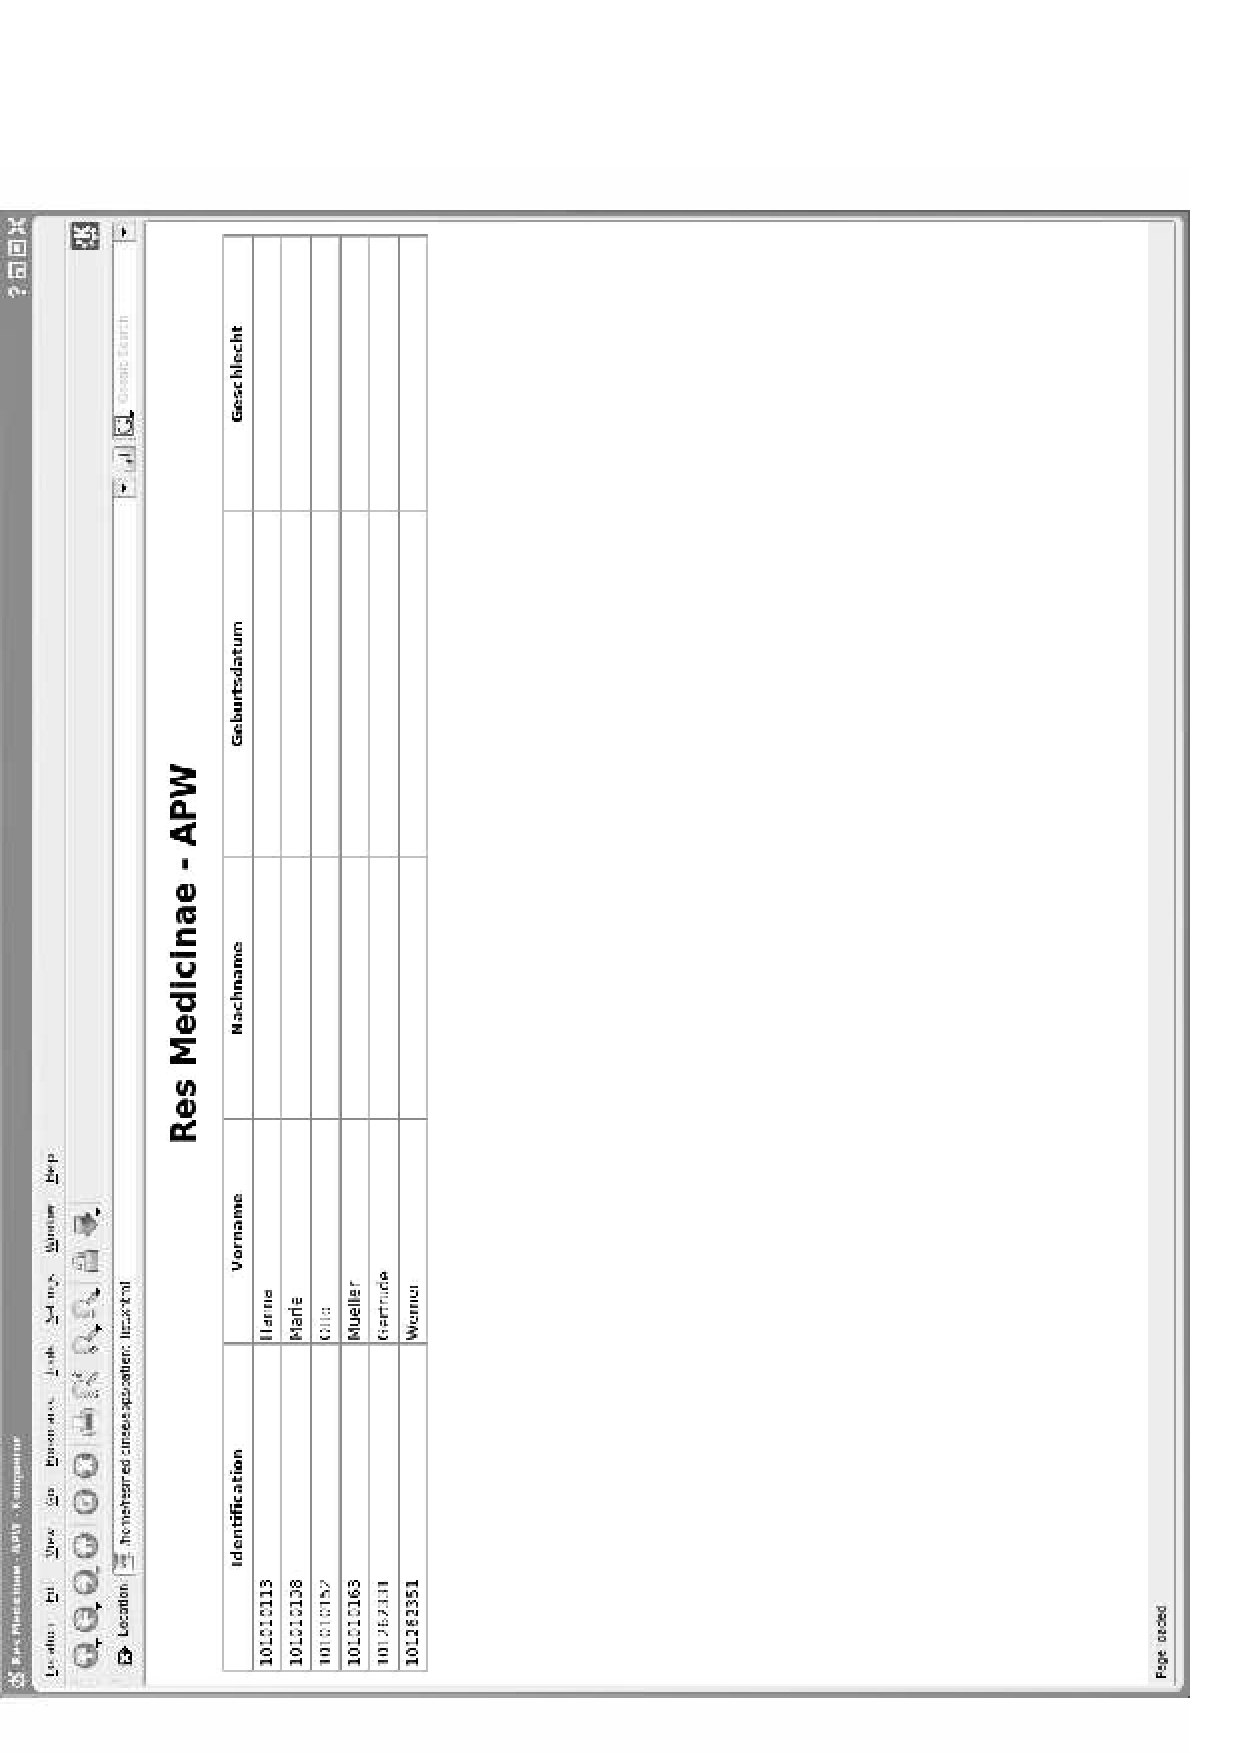
\includegraphics[scale=0.3,angle=-90]{graphics/web_user_interface.pdf}
        \caption{Web User Interface}
        \label{web_user_interface_figure}
    \end{center}
\end{figure}

\subsubsection{Example}

\begin{scriptsize}
    \begin{verbatim}
<part name="address_table" channel="file" abstraction="compound" model="wui/table.cybol">
    <property name="tag" channel="inline" abstraction="character" model="table"/>
    <property name="width" channel="inline" abstraction="character" model="100%"/>
    <property name="cellspacing" channel="inline" abstraction="integer" model="5"/>
    <property name="cellpadding" channel="inline" abstraction="integer" model="2"/>
    <property name="border" channel="inline" abstraction="boolean" model="false"/>
</part>
    \end{verbatim}
\end{scriptsize}

\subsubsection{Tag Property}

This property specifies the HTML tag to associate with the knowledge model.

\emph{required}

name=\texttt{'tag'}\\
abstraction=\texttt{'character'}\\
model=\texttt{'html' \vline\ 'head' \vline\ 'meta' \vline\ 'body' \vline\ 'table' \vline\ 'tr' \vline\ etc.}

\subsubsection{Xmlns Property}

This property specifies the XML namespace for the HTML page to be generated
from the WUI.

\emph{optional}, only for \emph{html} tag

name=\texttt{'xmlns'}\\
abstraction=\texttt{'character'}\\
model=\texttt{'http://www.w3.org/1999/xhtml'}

\subsubsection{HTTP-Equiv Property}

This property specifies the content type for the HTML page to be generated from
the WUI.

\emph{optional}, only for \emph{meta} tag

name=\texttt{'http-equiv'}\\
abstraction=\texttt{'character'}\\
model=\texttt{'content-type'}

\subsubsection{Name Property}

This property specifies the name of a meta data entry for the HTML page to be
generated from the WUI.

\emph{optional}, only for \emph{meta} tag

name=\texttt{'name'}\\
abstraction=\texttt{'character'}\\
model=\texttt{'author'}

\subsubsection{Content Property}

This property specifies the content of a meta data entry for the HTML page to
be generated from the WUI.

\emph{optional}, only for \emph{meta} tag

name=\texttt{'content'}\\
abstraction=\texttt{'character'}\\
model=\texttt{'Generated by CYBOI'}

\subsubsection{Align Property}

This property specifies the alignment of the HTML heading.

\emph{optional}, only for \emph{h1..6} tag

name=\texttt{'align'}\\
abstraction=\texttt{'character'}\\
model=\texttt{'left' \vline\ 'right' \vline\ 'center'}

\subsubsection{Width Property}

This property specifies the width of the HTML table.

\emph{optional}, only for \emph{table} tag

name=\texttt{'width'}\\
abstraction=\texttt{'character'}\\
model=\texttt{table width}

\subsubsection{Cellspacing Property}

This property specifies the spacing between the cells of the HTML table.

\emph{optional}, only for \emph{table} tag

name=\texttt{'cellspacing'}\\
abstraction=\texttt{'character'}\\
model=\texttt{space between cells in pixels}

\subsubsection{Cellpadding Property}

This property specifies the space between an HTML table cell's border and its
content.

\emph{optional}, only for \emph{table} tag

name=\texttt{'cellpadding'}\\
abstraction=\texttt{'character'}\\
model=\texttt{space between cell border and content}

\subsubsection{Border Property}

This property specifies the width of the HTML table's border.

\emph{optional}, only for \emph{table} tag

name=\texttt{'border'}\\
abstraction=\texttt{'character'}\\
model=\texttt{table border width}

\subsubsection{HRef Property}

This property specifies the reference (link) to be invoked when activating the
HTML element.

\emph{optional}, only for \emph{a} tag

name=\texttt{'href'}\\
abstraction=\texttt{'character'}\\
model=\texttt{an HTML reference}
